%% Latex template for PhD dissertation or MS thesis
%% Electrical and Computer Engineering Department
%% Brigham Young University
%% Last Modified:  March 2012

\documentclass[12pt]{report}
\usepackage{multirow}

%%%%%%%%%%%%%%%%%%%%%%%%%%%%%%%%%%%%%%%%%%%%%%%%%%%%%%%%
%  Setup BYU thesis format
%%%%%%%%%%%%%%%%%%%%%%%%%%%%%%%%%%%%%%%%%%%%%%%%%%%%%%%%%
\usepackage{byustyle}
% Setup the byu style sheet
\byustylesetup{
	%
	%isdissertation = true,           % Uncomment this if you're doing a PhD dissertation
	%etdsubmission = true,            % Uncomment this if you're compiling it for ETD submission
	singlepageabstract = true, % Comment this out if your abstract is multiple pages
	singlepageacknowledgements = true, % Uncomment this if your Acknowledgements is multiple pages
	%
	% Definitions of names needed in thesis/dissertation
	deptname          = Department of Linguistics and English Language,
	collegename       = College of Humanities,
	committeechairman = Deryle Lonsdale,
	committeemembera  = Cynthia Hallen,
	committeememberb  = Alan Melby,
	committeememberc  = Michael Bush,
	%committeememberd  = Firstname Mi. Lastname,                     % PhD Only
	graddate = June 2016,  % Leave commented for current month and year
	%copyrightyear = 2012,      % Leave commented for current year
	% uncomment the keywords for a dissertation
	keywords         = {tokenization, lexing, morphological analysis},
	%
	% Uncomment to shorten for proofreading purposes
	noabstract = true,         % Don't show the abstract page
	%nouniversitypages = true,  % Don't show any of the "university pages"
	noacknowledgements = true, % Don't show the Acknowledgements page
	%notableofcontents = true,  % Don't show the Table of Contents
	nolistoffigures = true,    % Don't show the List of Figures
	nolistoftables = true,     % Don't show the List of Tables
	%notocandlists = true,      % Don't show the Table of Contents, List of Figures, or the List of Tables
	%noheaderatall = true,      % Don't show any of the BYU Thesis header pages
}
%%%%%%%%%%%%%%%%%%%%%%%%%%%%%%%%%%%%%%%%%%%%%%%%%%%%%%%%
%  END:  Setup BYU thesis format
%%%%%%%%%%%%%%%%%%%%%%%%%%%%%%%%%%%%%%%%%%%%%%%%%%%%%%%%%

%%%%%%%%%%%%%%%%%%%%%%%%%%%%%%%%%%%%%%%%%%%%%%%%%%%%%%%%
%  Include other \usepackage{} statements here.
%    Add one package at a time.
%    Warning:  Some packages are not compatible with byuthesis.sty
%%%%%%%%%%%%%%%%%%%%%%%%%%%%%%%%%%%%%%%%%%%%%%%%%%%%%%%%%
%\usepackage[normalmargins]{savetrees} % prints smaller to save trees (draft only)
\usepackage{amsmath,amssymb} % math definitions
\usepackage{graphicx}        % for figures
\usepackage{subfigure}       % for figures with multiple subfigures
\usepackage{setspace}        % so all the captions will be single spaced

\graphicspath{ {figures/} }

%%%%%%%%%%%%%%%%%%%%%%%%%%%%%%%%%%%%%%%%%%%%%%%%%%%%%%%%
%  END: Include other \usepackage{} statements here.
%%%%%%%%%%%%%%%%%%%%%%%%%%%%%%%%%%%%%%%%%%%%%%%%%%%%%%%%%

%%%%%%%%%%%%%%%%%%%%%%%%%%%%%%%%%%%%%%%%%%%%%%%%%%%%%%%%
% For doing bookmarks in the PDF file
%%%%%%%%%%%%%%%%%%%%%%%%%%%%%%%%%%%%%%%%%%%%%%%%%%%%%%%%%
% For more info, see:
% http://www.geocities.com/kijoo2000/latex2pdf.pdf
% http://www.tug.org/applications/hyperref/manual.html
\usepackage[backref,pagebackref,plainpages=false]{hyperref}
\hypersetup{
	 breaklinks   = false, % Allow link text to break across lines (default=false).
	 linktocpage  = false, % make page number, not text, be link on TOC, LOF and LOT
	 colorlinks   = false, % Color the text of links (true) or put color frames over
				  % the links (false).
	% NOTE: if you need to use a dvi->ps->pdf path for things like PSTricks, you
	% may find that commenting out the next line is necessary.
	pdfborder    = 001,   % sets the default for pdf links                      
	pdfstartview = {FitH},  % Set the startup page view. Possible options are:
							% FitH: Fit whole width of page
							% FitV: Fit whole height of page
							% FitB: Fit whole �Bounding Box� page
							% FitBH: Fit whole width of �Bounding Box� of page
							% FitBV: Fit whole height of �Bounding Box� of page
	bookmarksnumbered  = true, % Put section numbers in bookmarks (default=false)
	bookmarksopen      = true, % Open up the bookmark trees (default=false).
	bookmarksopenlevel = 1, % Level to which bookmarks are open (default=\maxdimen).
	bookmarkstype      = toc, % Specify which toc file to mimic (default=toc).
	pdfpagemode        = {UseOutlines}, %  Specify how document starts when opened ({None}).
										% Possible options are:,
										% None: Neither bookmarks nor thumbnails are visible.
										% UseOutlines: Bookmarks are visible.
										% UseThumbs: Thumbnails are visible.
										% FullScreen: Full-screen mode
	 pdftitle    = {A Hybrid Approach to Cross-Linguistic Tokenization: Morphology with Statistics},
	 pdfauthor   = {Logan Kearsley},
	 pdfcreator  = {Logan Kearsley},
	 pdfsubject  = {Logan Kearsley's Master's Thesis},
	 pdfkeywords = {Master's Thesis, BYU}
}

%%%%%%%%%%%%%%%%%%%%%%%%%%%%%%%%%%%%%%%%%%%%%%%%%%%%%%%%
%  END: For doing bookmarks in the PDF file
%%%%%%%%%%%%%%%%%%%%%%%%%%%%%%%%%%%%%%%%%%%%%%%%%%%%%%%%%

%%%%%%%%%%%%%%%%%%%%%%%%%%%%%%%%%%%%%%%%%%%%%%%%%%%%%%%%
%                Macros
%  Define macros here
%%%%%%%%%%%%%%%%%%%%%%%%%%%%%%%%%%%%%%%%%%%%%%%%%%%%%%%%%
\def\proof{\noindent{\it Proof: }}
\def\QED{\mbox{\rule[0pt]{1.5ex}{1.5ex}}}
\def\endproof{\hspace*{\fill}~\QED\par\endtrivlist\unskip}
%
\newcommand{\norm}[1]{\left\|#1\right\|}
\newcommand{\abs}[1]{\left|#1\right|}
\newcommand{\defeq}{\stackrel{\triangle}{=}}
\newcommand{\re}{\mathbb{R}} % real numbers
\newcommand{\OMIT}[1]{{}} % omit sections of text
\newcommand{\pd}[2]{\ensuremath{\frac{\partial #1}{\partial #2}}} % partial derivative

%%%%%%%%%%%%%%%%%%%%%%%%%%%%%%%%%%%%%%%%%%%%%%%%%%%%%%%%%
%                End Macros
%%%%%%%%%%%%%%%%%%%%%%%%%%%%%%%%%%%%%%%%%%%%%%%%%%%%%%%%%

% To only print a few chapters without changing the reference numbers,
% uncomment the chapters you want
\includeonly{litreview,methodology}

%%%%%%%%%%%%%%%%%%%%%%%%%%%%%%%%%%%%%%%%%%%%%%%%%%%%%%%%%
% Start Document
%%%%%%%%%%%%%%%%%%%%%%%%%%%%%%%%%%%%%%%%%%%%%%%%%%%%%%%%%

\begin{document}

% Define Title & Author
\title{A Hybrid Approach to Cross-Linguistic Tokenization: Morphology with Statistics}
\author{Logan R. Kearsley}

% For displaying the BYU Thesis header
% This command assumes that there are documents called abstract.tex and
% acknowledgements.tex that will be included in the header
\showBYUHeader


% Include chapters of the thesis here:
% each chapter should be in a file with a .tex extension and the text
% of the file should begin with \chapter{Chapter Title}, followed
% by the text of the chapter.
\chapter{Introduction}

One of the most basic and yet often overlooked problems in natural language processing (NLP) is word boundary detection, or tokenization. Identifying words is a critical preprocessing step before almost any other work can be done with text: frequency counting, part-of-speech tagging, parsing, etc.
In many languages, this is far from trivial. The standard orthographies for languages as diverse as Ancient Greek and Latin, and modern languages like Thai, Chinese, and Japanese, lack spaces or any other explicit indicator of word boundaries. This often results in ambiguity about the proper grouping of characters into words, and difficulty in identifying the boundaries of unknown words.

Substantial research has been done in text segmentation for languages like Chinese \cite{peng04} and Japanese \cite{suzuki00}. The highest-performing systems all use a hybrid approach, incorporating both statistical knowledge to predict probable word boundaries, and access to lexicons to identify known words. Unfortunately, the specific algorithms used are often drastically different, and bespoke tokenizers are typically built on a language-by-language basis. Even in English and other languages that use whitespace in writing, there are numerous edge-cases, such as clitic and punctuation separation, which must be handled with special rules on a per-language basis. In developing software for searching, analyzing, or teaching multiple languages, or supporting natural-language based user interfaces, the complexity of developing separate systems to support equal levels of computer-enhanced interactivity for every desired language quickly becomes impractical. This severely limits both the number of languages that can be supported in any given application and the level of functionality available for each language. Given that the human ability to successfully read any natural language provides an existence proof that a generalized segmentation system (as implemented in the human mind) is possible, it is reasonable to investigate the feasibility of a language-agnostic segmentation system that could be easily integrated into larger natural language processing systems.

In order to make NLP applications more accessible in a wider variety of languages, I am developing a generalizable framework for tokenization which can be easily adapted to any given language. The general tokenization problem can be broken down into a few generic parts, regardless of the language involved: a hypothesis generator, which makes use of both a morphological recognizer encoding lexical knowledge and a statistical model or models, and a selector, which identifies the best hypothesis. Even if a single master system cannot be used for every language, decomposing the problem in this way should allow for replacing only certain parts and reusing others, as long as the replacement modules conform to a standard interface.

For the purposes of this thesis, I have focused only on the hypothesis generation stage. I identify promising lexical and statistical models and several methods of integrating them into a single unified hypothesis generator. I then test these systems them on corpora of native-speaker texts from three typologically dissimilar languages. The success of each hypothesis generation system is determined by three factors. These are:
\begin{enumerate}
	\item the consistency of the results across multiple languages, or the generalizability of the system, which encompasses the other two factors;
	\item how effective the system is at producing the correct hypotheses;
	\item how much work is left for the later hypothesis selection stage, measured in terms of the total number of hypotheses produced.
\end{enumerate}
\chapter{Review of Literature}

Prior to almost any other natural language processing task, the first task that must be done with any text is tokenization (also called segmentation, lexing, or word breaking)\textemdash~figuring out where the words (or other logical units) are. 

This problem is most obvious in the context of automatic speech recognition, where it is further necessary to convert continuous phonetic data into discrete phonemes. The standard solution in this context is to use Hidden Markov Models (HMMs) encoding the possible words of the language to transduce phonetic data into sequences of potentially-overlapping \textit{possible} phonemes and words~\cite{varile97}. The correct tokenization is obtained by applying the Viterbi algorithm over a pre-generated lattice of ``word hypotheses"~\cite{aubert94}, or by performing an on-line beam search over possible tokenizations as new possibilities are generated~\cite{paul94}.

% NOTE: tie on-line-iness into complexity requirements

If we set aside the issue of transducing phonetic data into discrete phonemes, however, the problem of identifying logical groups in a stream of discrete lower-level symbols still remains, and we can isolate this aspect of the problem by working with written text, assembling morphemes and words from a stream of graphemes. In general, tokenization of written text\footnote{In corpus studies, ``text" is often used to refer to any reification of language, be it spoken or written; here however, I will assume that ``text" refers only to written communication.} may be a harder problem than tokenization of speech since writing generally does not reflect spoken language losslessly, and fewer boundary clues (such as prosodic information) will be available. Nevertheless, the fact that reading is possible is itself proof that text-only tokenization can be done at useful levels of accuracy.

\section{Tokenization of English}
In English and many other languages, the problem of text tokenization is often considered trivial: simply split words on whitespace, which substitutes for many of the prosodic clues available in speech. Aken~\cite{aken11}, for example, studied the problem of tokenizing continuous English text with spaces removed, but only as a proxy for understanding human tokenization strategies more generally. While often good enough, however, the space-splitting approach is far from perfectly accurate. Even with perfectly clean data, this approach fails to account for:
\begin{enumerate}
	\item Word boundaries that correctly occur in the absence of whitespace (e.g., before punctuation, with specialized items like URLs, or simply due to typographical errors)
	\item Whitespace that may not indicate a relevant boundary in certain applications (e.g., spaces in compounds, idioms, and borrowed foreign-language phrases used as single logical lexical units).
\end{enumerate}
These complications can be dealt with in various ways, but only on an individual language-by-language basis. Even among languages that all use the Roman alphabet, significant differences in whitespace and punctuation conventions exist. The tokenization conventions for the Penn Treebank, for example, separate ``most punctuation"~\cite{treebank}, but depend on prior knowledge of sentence boundaries to help disambiguate final periods from periods indicating abbreviations and on English-specific knowledge about the structure of contractions and cliticized forms.

Aken's system relies purely on statistical information available within a single text to infer word segmentation. In particular, it keeps track of recurring sequences that recur with with frequency greater than a certain threshold as possible word types. It further keeps track of the transition probabilities between known sequences to determine the optimal path through a lattice of tokenization hypotheses~\cite{aken11}. This algorithm was tested against both randomly generated strings of words from a dictionary, and a small sample of natural English text, which revealed a weakness in identifying boundaries in sequences of multiple short words, such as ``in a"; this is a particular weakness shared by other statistical algorithms as well. This approach taken in isolation would likely perform poorly on a text containing a large number of hapax legomena\footnote{Types which occur exactly once in a corpus.}, which would pass the frequency threshold for recognition, making it potentially less suitable for languages with extensive productive morphology.

Aken's algorithm also depends on an implicit assumption about what the definition of a ``word" is: a fixed sequence of symbols that can occur multiple times. While this assumption may indeed be a useful one for vocabulary induction from unlabeled data, it is not necessarily the best definition of ``word" for all circumstances, especially across multiple languages. Additionally, there is ambiguity in the usage of ``word" to refer to a particular sequence of symbols, versus a particular instance of that sequence in a text. Unfortunately, per Islam~\cite{islam07}, no widely accepted definitions for what constitutes a ``word" exist, even within a single language, let alone cross-linguistically. Different native speakers often segment text in different ways, and the rate of agreement between human judges can be less than 80\%, making it impossible to construct a single ``gold standard" to evaluate results between systems that employ different conventions, whether implicit or explicit. For these reasons, it is often useful to dispense with the problem of defining a ``word" at all and, when exactness is required, to instead refer to \textit{types}, meaning specific abstract sequences of symbols, and \textit{tokens}, meaning specific instances of a type at specific locations in a text. Tokenization is thus the process of identifying meaningful tokens, however ``meaningful" is defined for a particular application in a particular language, and may cover items traditionally identified as ``words" as well as clitics, punctuation, and other errata. Note, however, that differences in conventions regarding what constitutes a meaningful token at a given level of analysis still require consideration during evaluation. The performance of tokenization algorithms is usually evaluated in terms of \textit{precision} and \textit{recall}; precision ($P$) is defined as the proportion of items in the output that are correct (i.e., which match items in the answer key), while recall ($R$) is defined as the proportion of correct items (i.e., entries in the answer key) which are in the output. Mathematically, these are given by
\begin{center}
	$P = \frac{\abs{O \cap K}}{\abs{K}}$ \\
	$R = \frac{\abs{O \cap K}}{\abs{O}}$
\end{center}
where $O$ is the set of output items and $K$ is the set of answer key items. Since it is often easy to obtain high performance on either measure individually (e.g., perfect recall can be achieved simply by guessing that every character boundary might be a token boundary), but difficult to achieve high performance on both, an additional measure, the \textit{F-score} is used to combine precision and recall and provide an estimate of overall performance. This is defined as
\begin{center}
	$F = \frac{2PR}{(P + R)}$
\end{center}

While his algorithm requires no prior knowledge of linguistic structure, Aken~\cite{aken11} does note that ``A shortcut [...] is to incorporate a ready-made dictionary that contains some or all of the words that the algorithm will encounter." This lexical-access approach is most clearly demonstrated by Norvig~\cite{norvig14}, who describes the use of a simple lexicon to recursively split a string into a known word and a suffix of remaining characters, using dynamic programming techniques to construct a lattice to avoid the inefficiency of recomputing overlapping segmentations for the same suffixes multiple times. Word-level n-gram frequency data is then used to extract the highest probability tokenization from the lattice. Norvig~\cite{norvig14} cites applications to Chinese, as well as to specialized genres of English, such as URLs, which are written without spaces as previously described.
Norvig's algorithm, however, is only as good as the dictionary\textemdash~it will fail on encountering out-of-vocabulary (OOV) words. This makes it less suitable for application to languages that have extensive productive morphology, such as Turkish, in which it may be literally impossible to encode the complete set of possible words in a finite dictionary, even before we account for the fact that new words appear constantly in living languages~\cite{islam07}. Although this overlaps somewhat with the weaknesses of Aken's algorithm, the potential benefits of a hybrid approach are already evident, as a strong statistical algorithm may make up for gaps in vocabulary.

\section{Orthographies Traditionally Lacking Whitespace}
Most practical work in text tokenization involves languages whose writing systems traditionally have no spaces or other written word breaks, such as Chinese, Japanese, or Thai. In these cases, as with the special rules for Treebank annotation, researchers develop separate tokenization systems on a per-language basis, often using substantially different approaches ~\cite{peng04}\cite{suzuki00}.

Peng, Feng, \& McCallum~\cite{peng04} developed a system for Chinese segmentation which recasts segmentation as a tagging problem using linear-chain conditional random fields (CRFs); every character is tagged as either a start-of-word character, or not. This is an inherently hybrid system, as the CRF models incorporate lexical knowledge in addition to lower-level statistics, which are used for probabilistic new-word detection. This provides the best of both worlds: the efficiency and accuracy improvements that lexical access entails, without the need to store the entire vocabulary, and allowing for the proper identification of unknown words as long as they do not exhibit structural characteristics too far removed from those used to create the statistical model (i.e., the normal morphographological\footnote{The written parallel to morphophonological.} structure of the language). Their model produced results ranging from ($P = 0.828$, $R = 0.870$, $F = 0.849\%$) to ($P = 0.953$, $R = 0.961$, $F = 0.957$) over eight tests on various corpora.

The state-of-the-art Japanese segmentation system by Kudo, Yamamoto, \& Matsumoto~\cite{kudo04} also makes use of CRFs to simultaneously achieve tokenization and morphological analysis by selecting the best path through a lattice of possible \textit{morpheme}-level tokenizations generated from a morphologically-aware dictionary. In fact, Kudo et al. were primarily motivated by the problem of morphological analysis of unlabelled text, for which automatic tokenization was merely an unavoidable first step when working with Japanese orthography. This builds on prior work by Asahara et al.~\cite{asahara00} and Uchimoto et al.~\cite{uchimoto01} on Japanese tokenization and morphanalysis using HMMs and Maximum Entropy Markov Models (MEMMs), respectively. Kudo et al.'s CRF model improved on both HMM and MEMM models due to the ability of CRFs to make use of a wider range of tagging features, including lexical information, providing additional evidence for the utility of hybrid segmentation approaches. They report results of ($P = 99.04\%$, $R = 98.88\%$, $F = 98.96\%$) and ($P = 99.03\%$, $R = 99.20\%$, $F = 99.11\%$) on two different corpora.

Choosing to work at the level of morphemes rather than words additionally removes many of the problems present in other systems with hapax legomena or OOV words. This requires, however, either the ability to re-synthesize complete words from morphemes, or an agreement with later stages of the NLP pipeline to define ``tokens" at the appropriate sub-word level. Where possible, however, the ability to achieve simultaneous tokenization and morphanalysis substantially improves efficiency and provides more contextual information to later stages of an NLP pipeline, such as syntactic parsing.

Suzuki, Brockett, and Kacmarcik~\cite{suzuki00}, in fact, took this one step further, by using a syntactic model to simultaneously select an optimal tokenization while producing a syntactic parse. Like Kudo et al.~\cite{kudo04}, Asahara et al.~\cite{asahara00} and Uchimoto et al.~\cite{uchimoto01}, they also use a ``word breaker" that performs simultaneous morphanalysis while producing a lattice of possible tokenizations. However, they eliminate the complication of collapsing the information in the lattice into a single unambiguous best token sequence. Instead, the lattice is used as the bottom level of a parsing chart, with the selection of the correct token sequence being a natural consequence of identifying the best syntax tree. They report results ranging from ($P = 97.4\%$, $R = 98.0\%$, $F = 97.7\%$) to ($P = 98.1\%$, $R = 98.5\%$, $F = 98.2\%$) on three corpora.

% I thought about adding references to ``Incremental Joint Approach to Word Segmentation, POS
% Tagging, and Dependency Parsing in Chinese", but it doesn't really cover anything new that's
% missing from any of the existing references, and I don't want to focus too much on Chinese
% when I'm not actually doing anything with Chinese.

In my own previous work~\cite{kearsley13}, I addressed the problem of efficient lattice generation with simultaneous morphanalysis using a finite-state transducer (FST) based on the KIMMO two-level morphology system~\cite{koskenniemi84}. This system runs in amortized constant time per-character. Hence, as each input character needs to be examined exactly once and in document order to determine which morphemes it could participate in, it generates a lattice of all possible sequences of known morphemes that could be extracted from an input stream in amortized linear time over arbitrary sized inputs~\cite{kearsley13}. Storing the lexicon as a finite-state transducer both saves a great deal of space and also allows recognition of a potentially infinite number of regularly derived or inflected words, though with some reduction in flexibility versus the CRF models. Compared to a fixed lexicon as used by Norvig~\cite{norvig14}, a morphological transducer suffers less from from the problem of encountering OOV tokens, but does not solve the problem completely; it will still encounter difficulty with unknown roots and other morphemes. This system was tested on English and Turkish, using synthetic corpora consisting of randomly-generated sequences of concatenated words, similar to the method used by Aken~\cite{aken11}. On corpora of known words, the system achieved ($P = 0.209435$, $R = 1$, $F = 0.346335$) for English and ($P = 0.164989$, $R = 1$, $F = 0.283246$) on Turkish.

The great advantage of this approach is that nearly any morphological model can be adapted to use in a simultaneous lexical-access based tokenizer (although it is optimized for FST-based models). In other words, the language model does not need to be developed with tokenization specifically in mind, and existing analyzers are reuseable, potentially saving a great deal of effort that would otherwise go into another bespoke, language-specific tokenization system. Additionally, this approach specifically supports on-line, real-time usage. While that feature is common (nearly obligatory, in fact) for speech processing, it is relatively rare in text tokenization~\cite{aken11}. The low precision scores are attributable to the fact that I focused only on lattice generation, as a clearly separate issue from path selection\textemdash~an approach I continue in this thesis. Prior to optimal path selection, the precision measure of a lattice generation system reflects the level of genuine morphological ambiguity present in the input.

\section{Psychological Modeling}

In addition to the NLP-oriented approach, the tokenization problem also arises in language acquisition: When hearing a new language that one does not know, how does a learner begin to identify new words to add to their mental lexicon? This clearly requires some generic mechanism (although of unknown and possibly great computational complexity) for inducing probable words boundaries (where contiguous sequences between two boundaries then constitute words) from unlabeled input. That humans are capable of this provides an existence proof of the technical possibility of language-agnostic tokenization.

While studying the ways that human minds may tackle tokenization is not guaranteed to produce the best possible artificial tokenization system since they may involve unnecessary complexity or require quantities of data infeasible to obtain for many NLP applications (in the same way that the best way to build an airplane is not to exactly copy a flapping bird's wing), studies of human psychological segmentation mechanisms do serve two useful purposes: They set a baseline against which errors can be measured, and they may provide an initial example implementation from which further engineering can draw~\cite{daland09}.

To establish a baseline of performance, it is sufficient to use manually-tagged corpora as a gold standard to test against; to provide an example implementation for re-engineering, it is important to have a reasonable psychological model of human speech segmentation. Daland~\cite{daland09} argues that both statistical predictive mechanisms and lexical access are necessarily involved in human segmentation, with contributions from each shifting over the language acquisition process: statistical mechanisms in order to guess at the boundaries around new unknown words and to determine the probability that a potential bounded sequence is in fact a new word, and lexical access to filter errors. Empirical evidence for the validity of this claim is provided by Islam~\cite{islam07}, who reports that many state-of-the-art NLP systems do in fact use hybrid approaches. Daland~\cite{daland09} further proposes that there are only two feasible error-correction conditions for the human tokenization system. The first is statistical over-recognition, where lexical access must filter out erroneously predicted word boundaries; the second is statistical under-recognition, where lexical access must be prepared to add statistically unlikely word boundaries. Logically, however, both may occur in any newly-developed system.

In either case, we can expect an improvement from merging statistical and lexicon-based methods. The set of correct word boundaries found by either method would not a priori be expected to form a subset of those found by the other; thus, their unions would be a larger set of correct boundaries. However, in the case of statistical under-recognition, we would expect a smaller contribution from statistical boundary prediction to the recognition of unknown words by lexicon-based methods. We would thus expect that statistical over-recognition would be the norm, and indeed, this is exactly the result obtained by Rytting~\cite{rytting04}.

\section{Simplified Statistical Models}

Revisiting the analogy of the airplane versus flapping bird wing, one is led to wonder whether statistical models might exist which are much simpler than CRFs or HMMs yet still in some sense ``good enough".  Brent \cite{brent99}, motivated, like Daland, by the study of first language acquisition, identified distribution regularities at the phoneme (or grapheme) level, such as segment-to-segment transition probabilities, to be useful indicators of word boundaries~\cite{brent96}. In later work, Brent~\cite{brent99} and Rytting~\cite{rytting04} both investigated simple character-level statistical cues that could be used as effective predictors of word boundaries during language acquisition, and for tokenization of text. The identification of such useful ``minimal information" predictors holds significant promise for developing simplifications of Daland's cognitive model~\cite{daland09} and further improving the performance of hybrid tokenizers.

While Brent~\cite{brent99} assumed that a prediction technique based on local comparisons (i.e., looking for significant differences between the values of a given statistical measurement between adjacent positions in the text), would be \textit{most} appropriate for identifying word boundaries, Rytting~\cite{rytting04} argued that this is guaranteed to under-predict due to the impossibility of correctly identifying common single-segment words, since the values of any two measurements in immediately adjacent positions cannot simultaneously be either significantly greater than or significantly less than each other. This echoes the problems with identification of small words encountered by Aken~\cite{aken11} with a significantly more complex model. Global comparisons are therefore needed to ensure maximum recall of correct boundaries.

Rytting~\cite{rytting04} tested the predictive power of two statistics based on Brent's work~\cite{brent99}: character-level transition probabilities, and character bigram mutual information scores, using both local and global comparisons for each. Rytting ~\cite{rytting04} showed that, on Greek text, a very simple mutual-information (MI) model outperformed the competing transition-probability models. He also showed that it was highly over-predictive on its own, and that using a global threshold for comparison was the most effective of the techniques that he tested, giving results of ($P = 43.9\%$, $R = 54.4\%$, $F = 48.6\%$) for identifying individual token boundaries. This is despite the fact that the threshold value of zero used in Rytting's study~\cite{rytting04} was chosen ``arbitrarily" with no justification attempted. Rytting's model, however, does also take into account the probability, based on a pre-annotated training corpus, that any particular bigram spans a known word boundary.

In my own previous work~\cite{kearsley14}, I applied the MI approach to English, testing the sensitivity of the model to the quantity of training data available for calculating bigram MI scores. In contrast to Rytting's supervised approach, however, I employed a further simplified, completely unsupervised algorithm which relied solely on MI scores calculated from the unannotated text of the Open American National Corpus (OANC) \cite{oanc}, consisting of samples from a variety of genres including transcribed speech, fiction, news, and technical writing. Additionally, in response to Rytting's claim that the zero threshold is ``arbitrary", I compared its performance with an alternative ``gap threshold" assignment method. In this approach, a model-specific threshold is dynamically selected by dividing bigrams into two clusters based on the largest gap between successive MI scores.

While the results are not directly comparable since our experiments involved different languages, the unsupervised zero-threshold MI approach produced better accuracies than Rytting's supervised approach~\cite{rytting04}, although it comes at a cost in recall\textemdash~($P = 56.4\%$, $R = 38.6\%$, $F = 45.8\%$). The gap threshold approach, on the other hand, showed high recall, but lower precision-\textemdash~(\_,\_,\_). I also found that, above a certain relatively small minimum size, results were not strongly dependent on the size of the training corpus. This, combined with the demonstrated efficacy of the unsupervised approach, means that the data required to build useful statistical word boundary prediction systems can be acquired cheaply, without the need for human annotation. Neither my nor Rytting's results, however, show recall scores close to 100\%, which, together with the early performance plateau, supports Daland's thesis that human tokenization must transition from primarily static-based to more lexical-access based methods during the learning process. While these extremely simple systems based on a single statistical measure (in this case, mutual information) do not have sufficiently good performance to use entirely on their own, their improvement over a random baseline is sufficient to justify investigating their use as heuristic filters to improve the performance of more complex hybrid word segmentation systems~\cite{kearsley14}.

\section{Path Selection Methods}
While my work sidesteps the problem of path selection, it is worth briefly reviewing what options are available. Suzuki et al.'s~\cite{suzuki00} parser-based approach, while highly effective, is also very heavyweight, and several simpler options exist for modular systems that separate lattice generation from path selection. Kudo~\cite{kudo04}, as justification for the need to incorporate lexical knowledge, cites accuracy of over 90\% using a simple longest-prefix matching algorithm, which simply assumes that the longest prefix of a string which is a known token is a correct token, and then restarts after that longest prefix to find the next token. It is unclear, however, whether the cited statistic applies only to Japanese, or cross-linguistically. Islam~\cite{islam07} also describes a ``maximal match" algorithm (with several variations for resolving ambiguities), which essentially consists of finding the longest substring that is a known token (regardless of whether or not it is a prefix of the text), and then proceeding to select the next longest known tokens in the remaining non-overlapping sections of text. Their particular modification, using type frequency and entropy measurements to resolve ambiguity between equal-length options, achieved ($P = 89.92\%$, $R = 94.69\%$, $F = 92.24\%$) in tests on the Brown corpus. This method is particularly useful in restricted settings where it is necessary to identify correct instances of certain types in desegmented text, but where complete tokenization and identification of unknown tokens is unnecessary; for example, a ``maximal match" algorithm is used in the TIARA\footnote{The Interactive Annotated Reader Application} \cite{cloe12} and Ayamel \cite{todd14} software developed by BYU's ARCLITE Lab in order to identify words and phrases that require annotations to be applied\textemdash~an application in which normal English tokenization conventions are completely unsuitable, as the relevant tokens are often large than single words and may contain spaces.
%I know of other instances where this is used for essentially the same purpose, but I'm not certain if I'm allowed to cite them or not due to NDAs
Norvig~\cite{norvig14} provides an approach which incorporates language-specific knowledge but is still relatively simple, calculating the most likely lattice traversal using n-gram probabilities, as noted above. Accurate results from this approach, however, depend on access to an extremely large training corpus (over 3 billion words in this case) to ensure that accurate statistics are available for all possible n-grams; the algorithm's performance is compromised when presented not merely with OOV tokens, but with previously unseen sequences of known tokens. The OOV token problem is partially addressed by model smoothing\textemdash~assigning a small default probability to any unknown token\textemdash~but can be significantly ameliorated by replacing the simple word n-gram model with a part-of-speech (POS) tag model, which can produce accurate statistics with a much smaller training corpus, since one tag sequence equates to several concrete word sequences. The tag-based approach is particularly attractive for use with systems that employ simultaneous morphanalysis, since POS information comes essentially ``for free".

\section{Lattice Generation with Morphology \& Statistics}

Regardless of the path selection algorithm used, the final results are only as good as their input. If a lattice generation step cannot produce all of the correct token boundaries as hypotheses, then no selection algorithm can produce the complete correct token sequence. On the other hand, a naïve conservative lattice generation algorithm could simply propose \textit{every} character boundary as a possible token boundary, in which case the correct sequence is guaranteed to exist somewhere, and could be found\textemdash~but only in a highly inefficient manner, as the lattice generator has provided no useful information to guide the search. A separate lattice generation algorithm can thus be rated both on how many correct hypotheses its output contains, and on how much work it requires of the succeeding path selection algorithm. In this context, lexicon-based tokenizers have an additional advantage over many pure statistical algorithms in that they inherently produce pairs of starting and ending boundaries for specific tokens; this significantly reduces redundancy compared to single-boundary tagging systems~\cite{kudo04} like those of Peng et al.,~\cite{peng04}, Brent~\cite{brent99}, or Rytting~\cite{rytting04}. In the worst case, these systems can require considering a number of token hypotheses proportional to the square of the number of individual boundary hypotheses, significantly slowing down the tokenization process.

Based on my previous work, I have built a series of hybrid lattice-generation systems implementing fundamentally language-agnostic lexical-access based and simple statistical algorithms, employing pre-existing morphological analyzers to provide language-specific lexical knowledge. I will show that these relatively simple models produce good results, improving on the performance of either lexical-access based or simple statistical methods alone. I will also demonstrate the generalizability of these algorithms across multiple languages that are orthographically and typologically (specifically, morphologically) dissimilar.
\chapter{Methodology}

\section{Data Collection \& Formatting}
I ran tokenization experiments on each of three languages\textemdash~Arabic, English, and Korean. This first required acquiring and pre-processing appropriate corpus data for testing, including annotations indicating the correct token boundaries to use as a gold standard.

Corpus data for Arabic came from the Arabic Treebank: Part 1 v 3.0~\cite{maamouri05}, consisting of 165,419 tokens of Modern Standard Arabic, where tokens include full words, clitics, and punctuation. Corpus data for English was came from a subset of the Open American National Corpus (OANC)~\cite{oanc}, consisting of 100,165 tokens, again including words, clitics, and punctuation. Corpus data for Korean came from data packaged with the KLEX morphological analyzer~\cite{han04}, itself a subset of the Korean Treebank, consisting of 41,024 tokens, including independent words, punctuation, and dependent suffixes. In each case, I converted all data into plain text in UTF-8 encoding.

Answer keys and tokenizer outputs were stored as lists of pairs of starting and ending indices for each token. I measured token boundary indices in terms of Unicode codepoints in order to abstract away the problem of defining a single "character" in the presence of Arabic vowel diacritics and Hangul syllabary combining characters. English token boundary locations as measured in codepoints were already available in the OANC annotations, and only had to be extracted and put into the list format. I calculated answer keys for Arabic and Korean by matching up sequential tokens in part-of-speech tagging files with their locations in the unannotated plain text. 

\section{Morphological Tokenization}
The simplest dictionary-based tokenization algorithm calculates all possible substrings of the input. Each substring is then checked against the dictionary and, if found, is added to the lattice of possible tokens. In order to reduce the incidence of unknown tokens and reduce the size of the lexicon that needs to be stored, the simple dictionary can be replace by a morphological analyzer to determine whether a given string is or is not a token. This is particularly important in languages, such as Turkish, with extensive productive morphology, in which most tokens will not appear in a standard dictionary.

This naïve approach to lattice generation is, however, highly inefficient; given that there are $n-m+1$ substrings of length $m$ in any string of length $n$, and we must check for tokens of all possible lengths (of which there are $n$), the algorithm requires $\sum_{m=1}^{n}(n-m+1)=\frac{1}{2}n(n+1)$ or O$(n^{2})$ time to produce all possible substrings, times a language-specific function $w(m)$ representing the time required to accept or reject a string of length $m$ to produce the lattice of possible tokens. If $w(m)$ is approximately linear (i.e., the amount of time it takes to accept or reject a possible token is, on average, proportional to the length of the token), this results in $\sum_{m=1}^{n}m(n-m+1)=\frac{1}{6}n(n+1)(n+2)$ or O$(n^{3})$ time required to produce all possible tokenizations of a given input\textemdash~ entirely unacceptable for on-line, real-time use.
In practice, however, while specific tokens may be unbounded in length, the highly non-random morphological structure of human languages means that most non-tokens will be rejected early since the probability of any randomly selected substring being a valid prefix of the language is inversely related to length. As a result, for long inputs, $w(m)$ is well approximated by a language-specific constant factor $k_w$ representing the average time (in terms of codepoints read) required to accept or reject a string as a valid token, resulting in O($n^{2}$) asymptotic complexity. This is still too slow for on-line applications, but some additional savings are possible if we know that there is an upper limit on the largest possible token in the dictionary; that reduces $m$ to an effective constant factor as well, rather than ranging to the arbitrarily large value of $n$ (the total size of the input). A similar, adaptive, version of that optimization was used by Norvig in his lexicon-based algorithm~\cite{norvig14}.

There is one fundamental problem with the naïve algorithm which causes repeated work: the rejection of a particular substring as a token says nothing about the status of any other substrings containing the first as a prefix. This results in the need to check each substring, which means that each codepoint is examined $n/2$ times\textemdash~once for each substring of which it is a part\textemdash~ thus generating the aforementioned $O(n^{2})$ time complexity under the assumption that $w(m)$ has some constant upper bound. However, if it is possible to accept or reject substrings as possible \textit{prefixes}\footnote{where ``prefix" in this case refers to any string of codepoints matching the beginning of a token, not to a morphological prefix} of valid tokens, then, after a substring is rejected as a possible prefix of any valid token, there is no need to check any larger substrings containing the first as a prefix. This reduces the number of operations that must be performed on each codepoint to be proportional to the level of morphological ambiguity at any point in the input, which, under the same assumption that let us treat $w(m)$ as an effective constant, approaches a constant average value on large inputs, rather than growing linearly with the size of the input. This gives us access to amortized linear-time performance without the need to artificially limit the maximum length of substrings that we will consider for token-hood.

Additional redundancy can be eliminated by remembering that a particular substring has already been accepted as a possible token prefix when considering the text that follows it. Given an analyzer that can only check complete strings all at once (which is the interface provided by most morphological analyzers), each codepoint must be examined at least once for every possible token (or not-yet-rejected prefix of a possible token) that overlaps that codepoint's position; if, however, the internal state of an analyzer that has already accepted a given token prefix can be saved, and incrementally updated with following codepoints rather than starting over from the beginning of that prefix every time we need to check the validity of a new, longer substring starting at the same position, the number of operations that must be performed per codepoint is reduced to become proportional to the number of \textit{groups} of valid token prefixes having different starting points that overlap that position. This does not provide any additional asymptotic improvements, but is a significant constant-factor savings.

Both of these optimizations can be naturally realized by encoding the morphological analyzer as a finite state machine (FSM), which can consume input one codepoint at a time, examining each codepoint exactly once. Transitioning to an accepting state of the automaton triggers the output of the current accepted token, but does not cause the automaton to terminate. Instead, it continues consuming more codepoints and emitting tokens at every accepting state until entering a failure state, indicating that the string consumed up to that point is no longer a valid prefix of any token, and thus no more tokens beginning in the same position are recognizable. Since the automaton consumes no more input after reaching a failing state, substrings containing rejected prefixes are never considered. Additionally, common prefixes are identified only once; the complete set of a maximal token and all possible prefix tokens (e.g., base forms missing suffixes, or components of compounds) are recognized in the same time as a single maximal token. Encoding a morphological analyzer as a pure FSM is not always convenient\footnote{E.g., pure finite-state approaches to morphology has well-known problems dealing with reduplication.}, but the same optimizations are available to any model that relies only on features that can be updated one codepoint at a time, and can thus be analyzed as a (potentially infinite) state machine with each codepoint consumed resulting in a transition to a discrete, recallable state. Even without the optimization that eliminates duplicate work on all prefixes of a maximal token, however, we can at least achieve the necessary linear-time performance with any model that can reject invalid prefixes.

In order to recognize possible tokens occurring as suffixes of maximal tokens (base forms missing prefixes, components of compounds, etc.) and to recognize tokens beginning at later points in the input stream, it is necessary to initialize a new instance of a morphological model, whether FSM-based or otherwise, (henceforth a ``recognizer") in its starting state at each point in the input stream. Every time a codepoint is consumed, it is thus fed into each of a cohort of recognizers that have not yet reached failure states. When processing first starts, the number of active FSMs grows linearly with the number of input codepoints consumed, as one is created for each codepoint. Recognizers will, however, be eliminated at a rate proportional to $k_w$ (the aforementioned average number of codepoints required to reject a string as a possible token) times the size of the cohort. This algorithm is illustrated in \ref{morphdiagram}. Eventually, the collection of active recognizers reaches an approximate steady state, with a uniform average cohort size over long stretches of input. The expected number of recognizers active at any given point in the input stream, and thus the number of operations that must be performed per codepoint, is thus proportional to $k_w$. Hence, we achieve $O(k_{w}n) = O(n)$ (linear) performance, allowing the production of all possible tokenizations of any input on-line and (if the constant factors are small enough) in real time. Additionally, as each recognizer in a cohort can be advanced independently, the algorithm is trivially parallelizable.

I implemented a generic morphological tokenizer in Python which reads input, builds a lattice, and manages cohorts of recognizer, and and which allows any concrete morphological analyzer to be plugged in to the system. Where necessary, I then wrote simple wrappers around the morphological analyzers for each language to ensure that they would present the proper FSM-like interface.
The output of each morphological experiment was saved in the form of a list of pairs of codepoint indices indicating the beginnings and ends of identified tokens\textemdash~ the same format used for the answer keys. This allowed the output stream to be replayed for use in hybrid experiments without needing to actually re-run the morphological tokenizer again, saving significant amounts of time and computational resources.

\begin{figure}
	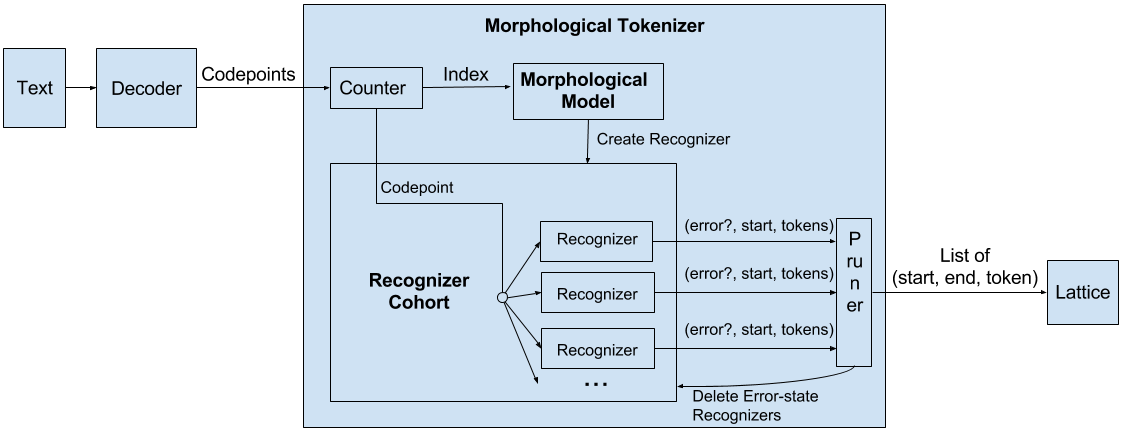
\includegraphics[width=\linewidth]{methodology/Morph}
	\caption{Morphological Tokenization}
	\label{morphdiagram}
\end{figure}

\subsection{Arabic}
I performed morphological tokenization of Arabic using the MADAMIRA morphological analyzer~\cite{pasha14}. MADAMIRA, unfortunately, does not expose an FSM network API, so it was necessary to collect complete candidate-token substrings to check all at once. Additionally, it does not provide any means of querying valid prefixes. In order to avoid quadratic or cubic runtime, which would make the experiment infeasible even on relatively short texts, extra rules were added to the interface connecting MADAMIRA to the generic tokenizer to reject strings satisfying certain conditions which I knew a priori could never result in valid prefixes. First, the interface would reject any string longer than 16 codepoints, as there were no tokens in the Arabic corpus greater than that length. Second, the interface would reject any string containing a whitespace codepoint, since I knew ahead of time that the MADAMIRA lexicon did not contain any tokens containing whitespace codepoints.
In other respects, however, MADAMIRA is almost \textit{too} sophisticated to effectively integrate with a tokenizer. In particular, MADAMIRA does not assume that the input will necessarily be a single word, and can analyze sentences with words in context; as a result, it does it's own word breaking (by some apparently undocumented method), and can return positive results for input containing more than one token. In order to account for this, I filtered MADAMIRA's output to accept only those strings which MADAMIRA identified as containing exactly one ``word". Additionally, MADAMIRA will ``helpfully" ignore extraneous punctuation, leading it to produce valid analyses for words with, e.g., parentheses attached, as well as for the actual words themselves. I could find no principled way to avoid these spurious analyses.

MADAMIRA is accessed via an HTTP interface, which introduces significant Input/Output overhead. In order to maximize CPU usage, I split the corpus into three parts processed by three simultaneous instances of the tokenizer, each accessing a single MADAMIRA server process.

\subsection{English}
I performed morphological tokenization of English with the Englex morphological description of English~\cite{antworthenglex} developed for PC-KIMMO~\cite{koskenniemi84}. This model was run on a modified version of PyKIMMO\footnote{A Python implementation of the KIMMO two-level morphology algorithm.} known as Stream-KIMMO~\cite{kearsley13}, which already has the appropriate FSM-like interface and required no adaptation. While the system runs in linear time, however, the original PyKIMMO implementation was highly inefficient, and introduced an enormous constant-factor slowdown, proportional to the size of the lexicon, due to simulating an FSM by dynamically calculating transitions and new states by iterating over the entire plain-text lexicon on every codepoint. Re-implementing the core of PyKIMMO to construct a real FSM was not a viable option, but I was able to introduce several efficiency improvements which sped up the algorithm by approximately a factor of five; still, the relative slowness of this analyzer limited the quantity of text that could be processed from the OANC within a reasonable time frame. The English morphological experiment was thus terminated after approximately four days.

\subsection{Korean}
I performed morphological tokenization of Korean using the KLEX morphological analyzer developed for the Xerox Finite-State Tools (XFST). KLEX was originally design to operate with input in either KSC-5601 or Unicode 1.0 encoding. In order to comply with modern versions of XFST, which only accept UTF-8 or Latin-1 encodings, and to enable it to work with the corpus which had been converted into UTF-8, I modified the KLEX source code to handle modern Unicode input. Fortunately, KLEX had been designed to transliterate Hangul into a modified Yale romanization for internal processing and back again; thus, updating it for modern encodings was a simple matter of running a search-and-replace on the file containing Hangul-Yale equivalencies to replace the old Korean codepoints with modern Unicode 8.0 UTF-8 codepoints.
Python bindings for the XFST library do exist which are supposed to directly expose the underlying FSM, allowing linear-time traversal. However, these tools have not been maintained, and I was unable to successfully install the software. Instead, I made use of a simpler Python API which exposes only the ``apply up" and ``apply down" functions of the morphological analyzer. As with MADAMIRA, I thus introduced special-case rules which rejected any string longer than 22 codepoints (again based on the maximum-length token known to exist in the corpus), and to reject any string containing whitespace, again based on prior knowledge that the KLEX lexicon contained no tokens containing whitespace.
KLEX has the ability to recognize certain suffixes and clitics in isolation, if they are prefixed with the tag ``\^{}DEP+" to indicate their status as bound (dependent) morphemes. Thus, in order to account for at least some possible variation in tokenization conventions, I ran two experiments with the morphological tokenizer on Korean: one which ignored dependents, and one which checked every possible token alone and with ``\^{}DEP+" prefixed.

\section{Statistical Tokenization}
In order to create a predictive model for statistical tokenization, mutual information (MI) scores were first compiled for every pair of codepoints present in each corpus. For this purpose, MI is given by the formula $\log_2(\frac{P(a,b)}{P(a)P(b)})$, where $a$ and $b$ are adjacent codepoints, $P(x)$ is the probability of encountering a given codepoint $x$ at any position, and $P(a,b)$ is the joint probability of encountering the pair of codepoints $a$ followed by $b$ at any given position. Word boundaries were then predicted by testing the MI score of each codepoint pair in the corpora against a threshold value, as shown in \ref{statdiagram}. This trivially requires constant time per pair, and thus achieves the necessary $O(n)$ complexity for on-line usage, like the morphological algorithm.
Two different methods of calculating thresholds were used in different experiments: gap threshold, and zero threshold. In the gap threshold method, the largest gap between MI scores for a given languages was identified, and a model was created which predicts a token boundary between every pair of codepoints whose mutual information score falls below that gap. This encodes the intuition that there may be a significant clustering of codepoint pairs that can occur across token boundaries vs. codepoint pairs that tend to occur within tokens, and was previously found to produce extremely high recall with reasonable accuracy on English data~\cite{kearsley14}. In the zero threshold method, boundaries are predicted between every pair of codepoints whose MI score is less than or equal to 0, for all languages. This encodes the intuition that there may be a token boundary wherever the probability of encountering a codepoint in that position is less than the overall probability of encountering that codepoint in any position.
Contrary to Rytting's method~\cite{rytting04}, 2004), MI scores are used to make token boundary predictions directly, rather than weighting them against a known prior probability of a particular codepoint pair marking a token boundary as determined from training data. This simplification results in a completely unsupervised system, which makes it attractive for use in a hybrid system as it avoids increasing the amount of language-specific configuration needed beyond the dictionary or morphological model. Additionally, although in this case MI scores were calculated ahead of time to maximize performance, with either threshold-assignment method the model could be updated on-line, as in Brent's prior work~\cite{brent99}, during real-time processing of a large input stream.
As in the morphological experiments, the output of each statistical experiment was saved to allow replaying the output for hybrid experiments. Since the statistical methods only identify single boundaries between tokens, rather than pairs bounding the start and end of a token, the saved output in this case consists of only a single list of possible boundary indices.

\begin{figure}
	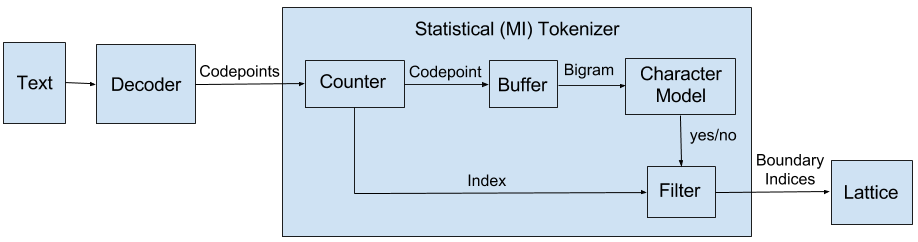
\includegraphics[width=\linewidth]{methodology/MI}
	\caption{Statistical Tokenization}
	\label{statdiagram}
\end{figure}

\section{Hybrid Tokenization}
I tested two methods of combining statistical and morphological methods to produce an improved hybrid tokenization system: ``filtering" and ``filling". Each of these was run with the output of both zero-threshold and gap-threshold statistical experiments, for a total of four hybrid experiments.

The filtering method is an attempt to improve system performance on precision by only initiating a new recognizer to add to the active cohort in the morphological tokenizer at indices where the statistical model indicates a token boundary is likely. This should eliminate spurious tokens that appear as suffixes of other tokens. This approach was simulated by constructing a new stream of (start, end) index pairs from stored morphological output including only those pairs in which the start index exists in the stored statistical data.

The filling method is an attempt to improve performance on recall and address the limitations of lexical-access based tokenization methods (including morphological tokenizers). This approach uses statistical predictions to fill in gaps of unanalyzed codepoints between tokens identified by the morphological model. This was simulated by identifying spans of codepoints not covered by any (start, end) pair in the morphological output, and filling them in with all (start, end) pairs that could be constructed from the predictions of the statistical models over those spans. One downside of this method is that, while it should run in amortized linear time in most cases, it does have worst-case quadratic performance on pathological inputs where the morphological model recognizes no possible tokens.

\begin{figure}
	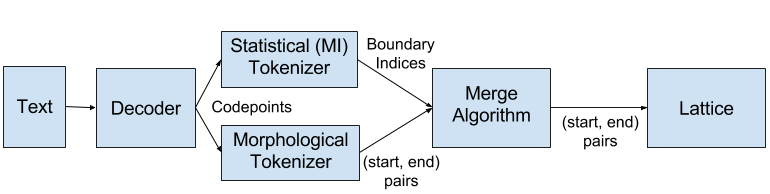
\includegraphics[width=\linewidth]{methodology/Hybrid}
	\caption{Hybrid Tokenization}
	\label{hybriddiagram}
\end{figure}

\section{Evaluation}
I evaluated all seven experiments on recognition of starting boundaries, ending boundaries, total individual boundaries, and matched pairs, representing specific tokens.

Since statistical predictions do not distinguish starting boundaries from ending boundaries, the precision measures for starting and ending boundaries considered individually are skewed, as they were determined by the total number of correctly-predicted boundaries that are starting (or ending) boundaries over the total number of undifferentiated boundaries predicted. This makes comparisons with the precision and F-scores for other methods slightly suspect. Recall, however, could be calculated normally for start and ending boundary predictions, and all three measures were calculated normally for the total set of individual boundaries. Token recall was based on the number of (start, end) pairs in the answer key for which both starting and ending indices appeared in the statistical output. I omitted precision calculations for complete tokens since the lack of pairing information makes precision measures on an un-pruned lattice (containing token hypotheses derived from all possible pairs of undistinguished boundaries) almost useless\textemdash~ the number of possible hypotheses without pruning grows as the square of the input length, making precision measurements dependent almost entirely on the size of the input, rather than any inherent feature of the algorithm. In the absence of a precision value, F-score is also meaningless. In place of precision for complete tokens, I also evaluated statistical results on what fraction of all codepoint boundaries were identified as possible token boundaries; a lower score on this measure corresponds to a higher effective precision, in terms of reducing the amount of work required by later stages of an NLP pipeline.

For the morphological experiments, I calculated precision, recall, and F-score for all four types of output. Starting and ending boundary sets were merged into a single undifferentiated set to allow direct comparison on that measure with the purely statistical methods. With no generic method of controlling for the effects of differing effective token definitions between corpora and morphological analyzers, I obtained qualitative results by manual inspection of the lists of missed types and tokens for each language.

Since morphological tokenization depends on a morphological analyzer to identify lexical items and other valid tokens, the accuracy and recall of the morphological tokenizer in any particular language is dependent on the qualities of the analyzer available for that language. In particular, we can expect maximum accuracy and recall measurements when the definition of a 'token' used by the creator of a morphological analyzer is the same as the definition of a token used by the corpus annotator. Additionally, we can expect recall to be approximately bounded by the percentage of actual tokens in the corpus that are recognizable by the analyzer in isolation, with any missed tokens being restricted to those that are out-of-vocabulary for the analyzer.
In order to control for the quality of the analyzers used, I ran coverage tests to measure the fraction of tokens and types in the answer key that were recognizable by the analyzer for each language.

As in the morphological experiments, I calculated precision, recall, and F-score for starting boundaries, ending boundaries, total individual boundaries, and matched pairs for all hybrid experiments. I also calculated a reduction factor for the filter experiments, consisting of the total number of token boundaries output by the filtering algorithm divided by the number of boundaries present in the raw morphological output.
\chapter{Results \& Discussion}
\FloatBarrier

Overall system performance on boundary identification for all seven experiments on all three languages is summarized in \ref{bsumtable}. Since F-scores were not calculated for token identification on the pure statistical experiments, \ref{tsumtable} provides a summary of system performance on the remaining five experiments across all three languages.

These summary views show significant variability in F-score across languages on almost every experiment, with the notable exception of gap threshold boundary recognition (listed in \ref{bsumtable}). These summary numbers, while an important indicator of the range of performance that can be expected from this kind of system using off-the-shelf data sources, do not, however, account for variability in the performance of individual morphological models or mismatches between the effective token definitions used by the answer keys versus the tokenizer. Examining the raw precision and recall scores for each individual experiment provides much deeper insights.

\begin{table}
	\centering
	\begin{tabular}{ | c | c | c | c |}
		\cline{2-4}
		\multicolumn{1}{c|}{} & Arabic & English & Korean \\ \hline
		Morphological & 0.137505 & 0.346242 & 0.284924 \\ \hline
		Zero Filter & 0.087241 & 0.155838 & 0.057650 \\ \hline
		Zero Fill & 0.137448 & 0.074367 & 0.283966 \\ \hline
		Gap Filter & 0.137505 & 0.346242 & 0.142457 \\ \hline
		Gap Fill & 0.137448 & 0.074367 & 0.283966 \\ \hline
	\end{tabular}
	\caption{F-scores for token recognition}
	\label{tsumtable}
\end{table}

\begin{table}
	\centering
	\begin{tabular}{ | c | c | c | c |}
		\cline{2-4}
		\multicolumn{1}{c|}{} & Arabic & English & Korean \\ \hline
		Morphological & 0.257299 & 0.601582 & 0.511887 \\ \hline \hline
		Zero Threshold & 0.242313 & 0.280959 & 0.129573 \\ \hline
		Zero Filter & 0.309639 & 0.256445 & 0.214498 \\ \hline
		Zero Fill & 0.257201 & 0.153340 & 0.510694 \\ \hline \hline
		Gap Threshold & 0.606717 & 0.539698 & 0.668813 \\ \hline
		Gap Filter & 0.257299 & 0.601582 & 0.511884 \\ \hline
		Gap Fill & 0.257201 & 0.153340 & 0.510694 \\ \hline
	\end{tabular}
	\caption{F-scores for boundary recognition}
	\label{bsumtable}
\end{table}
\FloatBarrier

\section{Morphological Tokenization}
\FloatBarrier

The Korean morphological experiments surprisingly produced identical output when explicitly checking for dependent tokens and when and ignoring them. Thus, only one set of Korean results is shown.

\ref{rectable} shows the results of coverage tests for types and tokens for each morphological analyzer. The token recall rates for each language as shown in \ref{morphtable} closely track the token coverage rates of the respective analyzers, which indicates that, given a suitable morphological model, this approach to lattice generation does indeed generalize well across languages.

MADAMIRA, with the best coverage, failed to recognize only four types in the entire corpus, both of which were abbreviations in non-Arabic script. The unusually low coverage of ENGLEX is attributable to multiple factors. First, unlike the other two analyzers, ENGLEX did not recognize punctuation, which eliminates a large group of common types. A more significant contribution to ENGLEX's low performance, however, is due to arguable errors in the answer key, and hence errors in the annotations to the OANC. Specifically, a large number of the types which ENGLEX failed to recognize are things like ``alaska--are", ``bed-", or ``city--to"\textemdash~ agglomerations of one or more words and punctuation, which reasonably should be interpreted as multiple tokens. Both ENGLEX and KLEX, however, failed to identify over a thousand genuine word types genuinely present in the corpora. Neither ENGLEX nor KLEX correctly identified numerical tokens, and ENGLEX failed to recognize punctuation.

Precision scores, on the other hand, are far more variable. This is attributable to the level of genuine ambiguity recognized by the model, which is in part a feature of specific morphological analyzers but is also largely dependent on the real features of a language. English, with the highest token precision score, has a relatively low rate of smaller tokens occurring as substrings of larger tokens, which as attributable to the relatively isolating nature of English morphology compared to Arabic or Korean. Additionally, the English precision scores should in fact be a little higher, as some of the lack of precision derives from the English tokenizer correctly identifying individual words in the aforementioned agglomerations like ``city--to", which are missing from the answer key.

The extremely low precisions seen for Arabic in comparison to either English or Korean are easily explained by the nature of Arabic orthography- since short vowels are typically not written, this explodes the number of possible analyses that have to be considered for any given string of text, even compared to the large number of prefix analyses necessitated by Korean's agglutinative morphology. The results for this particular experiment, however, are likely unusually bad due to the overly-helpful nature of MADAMIRA as previously described; these low precision scores reflect the identification of strings like \novocalize``\RL{almtxhdah)}" as possible unique tokens, where MADAMIRA has ``helpfully" ignored a piece of punctuation which should have simply invalidated that string.

\begin{table}
	\centering
	\begin{tabular}{ c | c | c | c |}
		\cline{2-4}
		& MADAMIRA (Arabic) & ENGLEX (English) & KLEX (Korean) \\ \hline
		\multicolumn{1}{ |c| }{Types} & 0.999764 & 0.747059 & 0.924060 \\ \hline
		\multicolumn{1}{ |c| }{Tokens} & 0.999976 & 0.761174 & 0.941961 \\ \hline
	\end{tabular}
	
	\caption{Morphological Analyzer Recognition Rates}
	\label{rectable}
\end{table}

\begin{table}
	\centering
	\begin{tabular}{ cc | c | c | c |}
		\cline{3-5}
		& & Precision & Recall & F-score \\ \hline
		\multicolumn{1}{ |c }{ \multirow{4}{*}{Arabic} } &
		\multicolumn{1}{ |c| }{Start} & 0.073836 & 0.998735 & 0.137506 \\ \cline{2-5}
		\multicolumn{1}{ |c  }{} &
		\multicolumn{1}{ |c| }{ End } & 0.073836 & 0.998735 & 0.137506 \\ \cline{2-5}
		\multicolumn{1}{ |c  }{} &
		\multicolumn{1}{ |c| }{Total} & 0.147672 & 0.998735 & 0.257299 \\ \cline{2-5}
		\multicolumn{1}{ |c  }{} &
		\multicolumn{1}{ |c| }{Tokens} & 0.073835 & 0.998729 & 0.137505 \\ \hline \hline
		\multicolumn{1}{ |c }{ \multirow{4}{*}{English} } &
		\multicolumn{1}{ |c| }{Start} & 0.238051 & 0.808606 & 0.367818 \\ \cline{2-5}
		\multicolumn{1}{ |c  }{} &
		\multicolumn{1}{ |c| }{End} & 0.239844 & 0.814696 & 0.370588 \\ \cline{2-5}
		\multicolumn{1}{ |c  }{} &
		\multicolumn{1}{ |c| }{Total} & 0.477895 & 0.811651 & 0.601582 \\ \cline{2-5}
		\multicolumn{1}{ |c  }{} &
		\multicolumn{1}{ |c| }{Tokens} & 0.224087 & 0.761174 & 0.346242 \\ \hline \hline
		\multicolumn{1}{ |c }{ \multirow{4}{*}{Korean} } &
		\multicolumn{1}{ |c| }{Start} & 0.173279 & 0.988841 & 0.294884 \\ \cline{2-5}
		\multicolumn{1}{ |c  }{} &
		\multicolumn{1}{ |c| }{ End } & 0.172365 & 0.983624 & 0.293328 \\ \cline{2-5}
		\multicolumn{1}{ |c  }{} &
		\multicolumn{1}{ |c| }{Total} & 0.345644 & 0.986233 & 0.511887 \\ \cline{2-5}
		\multicolumn{1}{ |c  }{} &
		\multicolumn{1}{ |c| }{Tokens} & 0.167426 & 0.955441 & 0.284924 \\ \hline
	\end{tabular}
	\caption{Results for morphological tokenization}
	\label{morphtable}
\end{table}
\FloatBarrier

\section{Statistical Tokenization}
\subsection{Zero Threshold}
\FloatBarrier

\ref{zpredtable} shows the fraction of all codepoint boundaries which were identified as possible token boundaries in each language. Surprisingly, the prediction rates closely correspond to recall performance for each language\textemdash~ Korean, with the lowest prediction rate, also shows the lowest recall and F-scores, while English and Arabic and comparatively very close together.

There is remarkable similarity between all three languages on total boundary precision. Compared to my \cite{kearsley14} and Rytting's \cite{rytting04} prior results, however, these look quite bad. Since my previous experiments were in fact run on a different subset of the same larger corpus (OANC), this suggests that the similarity of results seen here may simply be coincidental. This approach, therefore, does not seem to generalize well either across languages or even across different corpora within the same language.

The usefulness of this method is thus determined by the level of overlap between it's predictions and those of morphological tokenization, which is addressed in the hybrid experiments.

\begin{table}
	\centering
	\begin{tabular}{| c | c | c |}
		\hline
		Arabic & English & Korean \\ \hline
		0.267130 & 0.209335 & 0.099916 \\ \hline
	\end{tabular}
	\caption{Prediction rate for Zero-threshold statistical tokenization}
	\label{zpredtable}
\end{table}

\begin{table}
	\centering
	\begin{tabular}{ cc | c | c | c |}
		\cline{3-5}
		& & Precision & Recall & F-score \\ \hline
		\multicolumn{1}{ |c }{ \multirow{4}{*}{Arabic} } &
		\multicolumn{1}{ |c| }{Start} & 0.162632 & 0.198899 & 0.178947 \\ \cline{2-5}
		\multicolumn{1}{ |c  }{} &
		\multicolumn{1}{ |c| }{ End } & 0.156655 & 0.191589 & 0.172370 \\ \cline{2-5}
		\multicolumn{1}{ |c  }{} &
		\multicolumn{1}{ |c| }{Total} & 0.319287 & 0.195244 & 0.242313 \\ \cline{2-5}
		\multicolumn{1}{ |c  }{} &
		\multicolumn{1}{ |c| }{Tokens} & - & 0.040725 & - \\ \hline \hline
		\multicolumn{1}{ |c }{ \multirow{4}{*}{English} } &
		\multicolumn{1}{ |c| }{Start} & 0.121669 & 0.137783 & 0.129225 \\ \cline{2-5}
		\multicolumn{1}{ |c  }{} &
		\multicolumn{1}{ |c| }{ End } & 0.266911 & 0.302261 & 0.283488 \\ \cline{2-5}
		\multicolumn{1}{ |c  }{} &
		\multicolumn{1}{ |c| }{Total} & 0.388580 & 0.220022 & 0.280959 \\ \cline{2-5}
		\multicolumn{1}{ |c  }{} &
		\multicolumn{1}{ |c| }{Tokens} & - & 0.046703 & - \\ \hline \hline
		\multicolumn{1}{ |c }{ \multirow{4}{*}{Korean} } &
		\multicolumn{1}{ |c| }{Start} & 0.109952 & 0.042950 & 0.061771 \\ \cline{2-5}
		\multicolumn{1}{ |c  }{} &
		\multicolumn{1}{ |c| }{ End } & 0.286540 & 0.111930 & 0.160978 \\ \cline{2-5}
		\multicolumn{1}{ |c  }{} &
		\multicolumn{1}{ |c| }{Total} & 0.396492 & 0.077440 & 0.129573 \\ \cline{2-5}
		\multicolumn{1}{ |c  }{} &
		\multicolumn{1}{ |c| }{Tokens} & - & 0.006073 & - \\ \hline
	\end{tabular}
	\caption{Results for Zero-threshold statistical tokenization}
	\label{zstattable}
\end{table}
\FloatBarrier

\subsection{Gap Threshold}
\FloatBarrier

\ref{gpredtable} shows the fraction of all codepoint boundaries which were identified as possible token boundaries in each language. In one sense, this is clear evidence of generalization- in all three languages, a similar fraction of boundaries were identified. Unfortunately, this is makes the model very nearly useless for practical purposes. It fails to capture the unique structural features of each language's lexicon, and is thus little better than the brute-force case of hypothesizing that \textit{every} codepoint boundary is a possible token boundary. It is, in fact, worse than brute-force in one significant way: although the recall scores shown in \ref{gstattable} are very high, they are not 100\%, meaning that despite extreme levels of overprediction, the gap threshold statistical approach still missed some real token boundaries.

Given the marginal difference from hypothesizing every codepoint boundary, the precision scores (and thus F-scores) for this method are almost entirely determined by the average token length in each language. None of the languages tested have sufficiently distinctive bigram-level token-boundary statistics to prevent prediction of spurious boundaries internal to actual tokens, and, assuming a uniform distribution of predicted boundaries throughout the text, the number of spurious boundaries internal to an actual token is inversely related to the number of actual tokens in the text, and thus directly related to average token length.

The usefulness of this method is thus determined by the level of overlap between it's predictions and those of morphological tokenization, which is addressed in the hybrid experiments.

\begin{table}
	\centering
	\begin{tabular}{| c | c | c |}
		\hline
		Arabic & English & Korean \\ \hline
		0.999988 & 0.999945 & 0.999973 \\ \hline
	\end{tabular}
	\caption{Prediction rate for Gap threshold statistical tokenization}
	\label{gpredtable}
\end{table}

\begin{table}
	\centering
	\begin{tabular}{cc | c | c | c |}
		\cline{3-5}
		& & Precision & Recall & F-score \\ \hline
		\multicolumn{1}{ |c }{ \multirow{4}{*}{Arabic} } &
		\multicolumn{1}{ |c| }{Start} & 0.218421 & 0.999982 & 0.358530 \\ \cline{2-5}
		\multicolumn{1}{ |c  }{} &
		\multicolumn{1}{ |c| }{ End } & 0.217459 & 0.995580 & 0.356952 \\ \cline{2-5}
		\multicolumn{1}{ |c  }{} &
		\multicolumn{1}{ |c| }{Total} & 0.435880 & 0.997781 & 0.606717 \\ \cline{2-5}
		\multicolumn{1}{ |c  }{} &
		\multicolumn{1}{ |c| }{Tokens} & - & 0.9955628 & - \\ \hline \hline
		\multicolumn{1}{ |c }{ \multirow{4}{*}{English} } &
		\multicolumn{1}{ |c| }{Start} & 0.184808 & 0.999700 & 0.311948 \\ \cline{2-5}
		\multicolumn{1}{ |c  }{} &
		\multicolumn{1}{ |c| }{End} & 0.184812 & 0.999720 & 0.311954 \\ \cline{2-5}
		\multicolumn{1}{ |c  }{} &
		\multicolumn{1}{ |c| }{Total} & 0.369619 & 0.999710 & 0.539698 \\ \cline{2-5}
		\multicolumn{1}{ |c  }{} &
		\multicolumn{1}{ |c| }{Tokens} & - & 0.999621 & - \\ \hline \hline
		\multicolumn{1}{ |c }{ \multirow{4}{*}{Korean} } &
		\multicolumn{1}{ |c| }{Start} &0.253362 & 0.990502 & 0.403510 \\ \cline{2-5}
		\multicolumn{1}{ |c  }{} &
		\multicolumn{1}{ |c| }{ End } & 0.252121 & 0.985649 & 0.401533 \\ \cline{2-5}
		\multicolumn{1}{ |c  }{} &
		\multicolumn{1}{ |c| }{Total} & 0.505483 & 0.988075 & 0.668813 \\ \cline{2-5}
		\multicolumn{1}{ |c  }{} &
		\multicolumn{1}{ |c| }{Tokens} & - & 0.999663 & - \\ \hline
	\end{tabular}
	\caption{Results for Gap threshold statistical tokenization}
	\label{gstattable}
\end{table}
\FloatBarrier

\section{Hybrid Tokenization}
\subsection{Filtering}
\FloatBarrier

As could be predicted from the poor recall scores obtained in the zero-threshold statistical experiment, zero-threshold filtering resulted in reduced scores for almost all measures (listed in \ref{zflttable}) compared to pure morphological tokenization. There are slight improvements to ending boundary precisions for Arabic and Korean, and a slight increase in start boundary precision and token precision on English, but these are far outweighed by the reduced recall rates. Additionally, while useful for comparison with the pure statistical experiments, single-boundary precision is one of the least consequential performance metrics. What matters most are token precision and token recall; i.e., not merely correctly identifying individual boundaries, but correctly pairing them. While the filtering method did in fact achieve its goal of increasing precision, the fact that it only produced marginal improvement on token precision in one language, and had a severely negative effect on recall, makes this an essentially useless combination for practical purposes. The reduction rates, indicating potential run-time efficiency improvements, shown in \ref{zredtable}, while impressive, are thus unfortunately irrelevant.

\begin{table}
	\centering
	\begin{tabular}{| c | c | c |}
		\hline
		Arabic & English & Korean \\ \hline
		0.262744 & 0.135199 & 0.075932 \\ \hline
	\end{tabular}
	\caption{Filter Reduction for Zero-threshold}
	\label{zredtable}
\end{table}

\begin{table}
	\centering
	\begin{tabular}{ cc | c | c | c |}
		\cline{3-5}
		& & Precision & Recall & F-score \\ \hline
		\multicolumn{1}{ |c }{ \multirow{4}{*}{Arabic} } &
		\multicolumn{1}{ |c| }{Start} & 0.055894 & 0.198646 & 0.087241 \\ \cline{2-5}
		\multicolumn{1}{ |c  }{} &
		\multicolumn{1}{ |c| }{ End } & 0.186050 & 0.661221 & 0.290392 \\ \cline{2-5}
		\multicolumn{1}{ |c  }{} &
		\multicolumn{1}{ |c| }{Total} & 0.241944 & 0.429934 & 0.309639 \\ \cline{2-5}
		\multicolumn{1}{ |c  }{} &
		\multicolumn{1}{ |c| }{Tokens} & 0.055894 & 0.198646 & 0.087241 \\ \hline \hline
		\multicolumn{1}{ |c }{ \multirow{4}{*}{English} } &
		\multicolumn{1}{ |c| }{Start} & 0.263174 & 0.120861 & 0.165648 \\ \cline{2-5}
		\multicolumn{1}{ |c  }{} &
		\multicolumn{1}{ |c| }{End} & 0.423457 & 0.194469 & 0.266534 \\ \cline{2-5}
		\multicolumn{1}{ |c  }{} &
		\multicolumn{1}{ |c| }{Total} & 0.686630 & 0.157665 & 0.256445 \\ \cline{2-5}
		\multicolumn{1}{ |c  }{} &
		\multicolumn{1}{ |c| }{Tokens} & 0.247587 & 0.113702 & 0.155838 \\ \hline \hline
		\multicolumn{1}{ |c }{ \multirow{4}{*}{Korean} } &
		\multicolumn{1}{ |c| }{Start} & 0.099060 & 0.042924 & 0.059895 \\ \cline{2-5}
		\multicolumn{1}{ |c  }{} &
		\multicolumn{1}{ |c| }{ End } & 0.503204 & 0.218047 & 0.304255 \\ \cline{2-5}
		\multicolumn{1}{ |c  }{} &
		\multicolumn{1}{ |c| }{Total} & 0.602264 & 0.130486 & 0.214498 \\ \cline{2-5}
		\multicolumn{1}{ |c  }{} &
		\multicolumn{1}{ |c| }{Tokens} & 0.095346 & 0.041315 & 0.057650 \\ \hline
	\end{tabular}
	\caption{Results for Zero-threshold Filtering}
	\label{zflttable}
\end{table}

The results for gap threshold filtering show better performance, but no better utility. As shown in \ref{gredtable}, the level of overprediction produced by the gap threshold algorithm resulted in almost no actual filtering of the morphological outputs, meaning that the results are identical between these two methods for Arabic and English, and only tiny (less than $\pm.01\%$) differences for Korean. The extra time needed to calculate statistical information is thus, in this case, a performance loss rather than a gain.

Korean was the only language for which any filtering occurred at all. Unfortunately, even with the high level of overprediction in the gap threshold statistical results, the set of correct boundaries predicted by the gap threshold statistical algorithm did not completely overlap with the set of correct start boundaries predicted by the morphological algorithm, thus resulting in a decrease in recall compared to either method alone.

\begin{table}
	\centering	
	\begin{tabular}{| c | c | c |}
		\hline
		Arabic & English & Korean \\ \hline
		1.000000 & 1.000000 & 0.999973 \\ \hline
	\end{tabular}
	\caption{Filter Reduction for Gap threshold}
	\label{gredtable}
\end{table}

\begin{table}
	\centering
	\begin{tabular}{ cc | c | c | c |}
		\cline{3-5}
		& & Precision & Recall & F-score \\ \hline
		\multicolumn{1}{ |c }{ \multirow{4}{*}{Arabic} } &
		\multicolumn{1}{ |c| }{Start} & 0.073836 & 0.998735 & 0.137506 \\ \cline{2-5}
		\multicolumn{1}{ |c  }{} &
		\multicolumn{1}{ |c| }{ End } & 0.073836 & 0.998735 & 0.137506 \\ \cline{2-5}
		\multicolumn{1}{ |c  }{} &
		\multicolumn{1}{ |c| }{Total} & 0.147672 & 0.998735 & 0.257299 \\ \cline{2-5}
		\multicolumn{1}{ |c  }{} &
		\multicolumn{1}{ |c| }{Tokens} & 0.073835 & 0.998729 & 0.137505 \\ \hline \hline
		\multicolumn{1}{ |c }{ \multirow{4}{*}{English} } &
		\multicolumn{1}{ |c| }{Start} & 0.238051 & 0.808606 & 0.367818 \\ \cline{2-5}
		\multicolumn{1}{ |c  }{} &
		\multicolumn{1}{ |c| }{End} & 0.239844 & 0.814696 & 0.370588 \\ \cline{2-5}
		\multicolumn{1}{ |c  }{} &
		\multicolumn{1}{ |c| }{Total} & 0.477895 & 0.811651 & 0.601582 \\ \cline{2-5}
		\multicolumn{1}{ |c  }{} &
		\multicolumn{1}{ |c| }{Tokens} & 0.224087 & 0.761174 & 0.346242 \\ \hline \hline
		\multicolumn{1}{ |c }{ \multirow{4}{*}{Korean} } &
		\multicolumn{1}{ |c| }{Start} & 0.173275 & 0.988789 & 0.294875 \\ \cline{2-5}
		\multicolumn{1}{ |c  }{} &
		\multicolumn{1}{ |c| }{ End } & 0.172370 & 0.983624 & 0.293335 \\ \cline{2-5}
		\multicolumn{1}{ |c  }{} &
		\multicolumn{1}{ |c| }{Total} & 0.345644 & 0.986207 & 0.511884 \\ \cline{2-5}
		\multicolumn{1}{ |c  }{} &
		\multicolumn{1}{ |c| }{Tokens} & 0.167422 & 0.955389 & 0.284915 \\ \hline
	\end{tabular}
	\caption{Results for Gap threshold Filtering}
	\label{gflttable}
\end{table}
\FloatBarrier

\subsection{Filling}
\FloatBarrier

Surprisingly, the results for the filling hybridization method were identical for both zero-threshold and gap threshold statistics on all measures and across all three languages. Thus, only one set of unified results is shown, in \ref{filtable}. This suggests that, despite the vast differences in results between the zero-threshold and gap threshold statistical experiments on their own, both had identical outputs on spans of text for which the morphological algorithm alone could not identify any possible tokens. This pattern would have to break down given a morphological model with sufficiently low coverage, since results for zero-threshold filling and gap threshold filling must approach the results obtained from the pure statistical experiments in the limit where analyzer coverage goes to zero. But, even with token coverage as low as 76.12\%, as demonstrated by ENGLEX on the English corpus, the pattern still holds.

The identical results are fairly easy to explain for Arabic\textemdash~ with such high initial recall scores due to MADAMIRA's high coverage, there was very little left to fill in, and thus little room for potential variation in the output from different statistical algorithms.

The situation is more complicated for English and Korean, but suggests some commonality in the kinds of types that are likely to be left out of a morphological model. There are two (non-exclusive) obvious possibilities: First, they may be relatively small but frequent. Small gaps occupied by only one or a few small tokens minimize the opportunities for different statistical algorithms to differ, just as is the case with Arabic. Second, they may have uniquely distinguishing MI scores for their bounding bigrams. Specifically, they are types whose sets of bounding bigrams tend to have MI scores that are both less than or equal to zero, and less than the largest gap in MI scores for all bigrams in the language. Given that the largest gap is above zero for all three languages tested\footnote{Even without checking the specific numbers, this can be inferred from how much the gap threshold method overpredicts compared to zero threshold.}, this is equivalent to saying that the boundaries of common tokens unlikely to be recognized by morphological analyzers tend to have MI scores below zero, while the poor recall of the zero-threshold method indicates that many genuine tokens that are recognized by a morphological analyzer have boundary MI values above zero, but below the largest gap.

Both of these explanations appear to fail when confronted with examples like the aforementioned ``city--to", which make up a significant fraction of the missed tokens in English, and which is neither particularly short nor possesses particularly uncommon boundary characters. In fact, however, an eight-codepoint missed token like ``city--to" \textit{does not} constitute an eight-codepoint gap. This is because the morphological tokenizer \textit{does} identify tokens in that span\textemdash~ just not the one in the answer key. If those tokens were in fact legitimate, this would be a problem to be addressed by filtering, not filling.

In fact, the statistical algorithms are primarily identifying numbers and punctuation marks. Given that ENGLEX, as previously mentioned, misses both of these categories, while KLEX only fails on numbers, this explains why English is improved so much more than Korean, even though it does not quite reach parity: English simply has more of the relevant categories to make up, and results after statistical filling are limited by the number of remaining word tokens which the morphological analyzers cannot recognize.

Filling gaps of course comes at a cost in precision; this is seen most strongly in the English data, which is to be expected since the low coverage of the English analyzer provides more gaps to fill in, and thus more opportunities for overprediction. This of course results in a severe drop in F-score relative to pure morphological tokenization, and in fact the small reduction in precision more than offsets the small increase in recall for both remaining languages as well. Given that low recall makes identifying the correct tokenization from a lattice impossible, however, while low precision merely makes it more difficult, this is an acceptable tradeoff in most situations, since the precision scores for all languages are still much higher than would be obtained by the brute-force method.

\begin{table}
	\centering
	\begin{tabular}{ cc | c | c | c |}
		\cline{3-5}
		& & Precision & Recall & F-score \\ \hline
		\multicolumn{1}{ |c }{ \multirow{4}{*}{Arabic} } &
		\multicolumn{1}{ |c| }{Start} & 0.073804 & 0.998760 & 0.137451 \\ \cline{2-5}
		\multicolumn{1}{ |c  }{} &
		\multicolumn{1}{ |c| }{ End } & 0.073802 & 0.998735 & 0.137448 \\ \cline{2-5}
		\multicolumn{1}{ |c  }{} &
		\multicolumn{1}{ |c| }{Total} & 0.147607 & 0.998747 & 0.257201 \\ \cline{2-5}
		\multicolumn{1}{ |c  }{} &
		\multicolumn{1}{ |c| }{Tokens} & 0.073802 & 0.998735 & 0.137448 \\ \hline \hline
		\multicolumn{1}{ |c }{ \multirow{4}{*}{English} } &
		\multicolumn{1}{ |c| }{Start} & 0.041307 & 0.970349 & 0.079241 \\ \cline{2-5}
		\multicolumn{1}{ |c  }{} &
		\multicolumn{1}{ |c| }{End} & 0.041891 & 0.984056 & 0.080360 \\ \cline{2-5}
		\multicolumn{1}{ |c  }{} &
		\multicolumn{1}{ |c| }{Total} & 0.083198 & 0.977203 & 0.153340 \\ \cline{2-5}
		\multicolumn{1}{ |c  }{} &
		\multicolumn{1}{ |c| }{Tokens} & 0.038767 & 0.910667 & 0.074367 \\ \hline \hline
		\multicolumn{1}{ |c }{ \multirow{4}{*}{Korean} } &
		\multicolumn{1}{ |c| }{Start} & 0.172582 & 0.989619 & 0.293908 \\ \cline{2-5}
		\multicolumn{1}{ |c  }{} &
		\multicolumn{1}{ |c| }{ End } & 0.171826 & 0.985285 & 0.292621 \\ \cline{2-5}
		\multicolumn{1}{ |c  }{} &
		\multicolumn{1}{ |c| }{Total} & 0.344408 & 0.987452 & 0.510694 \\ \cline{2-5}
		\multicolumn{1}{ |c  }{} &
		\multicolumn{1}{ |c| }{Tokens} & 0.166744 & 0.956141 & 0.283966 \\ \hline
	\end{tabular}
	\caption{Results for Filling- Both Thresholds}
	\label{filtable}
\end{table}
\chapter{Conclusions \& Future Work}

Precision scores \hl{for tokenization} are highly sensitive to the details of a specific language's morphology and orthography. On the other hand, morphological tokenization generalizes well across the three languages I tested in terms of recall. In each case, recall scores are limited by the quality of the morphological analyzer used. Additionally, a simplified statistical model using character bigram mutual information scores with a zero threshold was effective at identifying unknown tokens like numbers and punctuation marks, which are likely to be left out of typical morphological analyses lexicons. This significantly improves recall performance in a hybrid tokenizer across multiple languages as well, even though the statistical approaches do not produce practical results in isolation.

The simplified statistical models employed for these experiments did prove useful for improving the performance of a hybrid tokenizer in a limited domain. More complex models, however, are needed to precisely identify unknown words whose boundary statistics are too similar to other words for MI scores to reliably distinguish. Additional research is also warranted on higher-recall statistical models that maintain reasonable precision to improve filtering efficiency. In principle, separate statistical models tuned for the different use cases could be employed for simultaneous filtering and filling, with an effective filter providing more opportunity for filling model to act by removing spurious morphological analyses and thus correctly identifying more spans as unknown.

While I achieved good results on Arabic, English, and Korean, these three languages do not cover the whole spectrum of variation seen in scripts for natural languages. A better picture of the generalizability\textemdash or limits thereof\textemdash of these algorithms could be obtained by testing on additional languages like Turkish (which is highly agglutinative and alphabetic), Thai (which uses an alphasyllabary with no spaces), Japanese, and Chinese.
Japanese is particularly interesting for the use of multiple scripts simultaneously, with transitions between kanji and hiragana providing significant token-boundary clues which may be easily picked up by a statistical model. Similarly, it would be useful to test on English corpora which include tokens that contain spaces, such as open compounds, borrowings, and idiomatic phrases. ENGLEX has some of these in its lexicon, but the answer keys derived from OANC annotations do not recognize them. Being able to evaluate the morphological tokenizer against an answer key whose tokenization conventions more closely match those of the analyzer's lexicon would improve the case for using this method over simple whitespace splitting even in languages (like English) which do use whitespace for the majority of token boundaries.

Additional small improvements to recall could be made by addressing the problem of overlapping tokens. This is most easily demonstrated by ambiguity in English periods\textemdash in a sentence like ``The Peloponnesian War concluded in 404 B.C.", the final period is both a part of the token ``B.C.", and an independent token marking the end of the sentence\textemdash two tokens overlap by a single character. Various forms of non-concatenative morphology or sandhi can create other cases where it is clear that there are multiple tokens, but not clear where precisely one token ends and another begins. This is difficult to handle when tokens are tied to specific positions in the input stream, but would be sidestepped if the data structure used to represent a lattice could preserve the logical ordering of tokens independent of their positions in the input stream.

Of course, having identified a cross-linguistically useful lattice generation algorithm, the next step in the pipeline is identifying a cross-linguistically useful path selection algorithm to match with it. Building on the work of Suzuki et al. in Japanese \cite{suzuki00}, it should be possible to design a generic on-line probabilistic parser which would then only require input of a language-specific syntactic model to do simultaneous tokenization, morphanalysis, part-of-speech tagging, and parsing, employing both bottom-up and top-down information at every stage. This would be more complicated, but still doable, given a lattice in which tokens are topologically sorted, but missing a consistent connection to input indices. Given the relative complexity of developing usefully-complete syntactic models, however, there is of course room for exploring the cross-linguistic applicability of shallower statistical models, like the smoothed token n-grams used by Norvig \cite{norvig14} or POS-tagging models (which, like syntactic models, would also assist in disambiguation of tokens with multiple morphological analyses). A slightly more exotic approach would be determining most-likely paths based on word association models like those produced by word2vec \cite{mikolov13}. This would pair particularly well with the morphological algorithm's ability to extend recognition to logical tokens like idiomatic phrases and open compounds which contain spaces.

%%%%%%%%%%%%% begin Bibliography %%%%%%%%%%%%%%%%%
\phantomsection %Forces a new section prior to setting the bibliography reference point
\bibliographystyle{IEEEtran}
\addcontentsline{toc}{chapter}{Bibliography}
\bibliography{refs}

% Bibliographies are best created and maintained using BibTeX
% To use Bibtex, create a bibliography file, e.g., refs.bib
% The sample file sources.bib shows examples of different
% bibliographic entries.
% The bibliography is created by executing:
%  1.  latex, 2. bibtex, 3. latex, 4. latex
%%%%%%%%%%%%%%%% end Bibliography %%%%%%%%%%%%%%%%%

%Included because WinEdit is RETARDED and it needs it for Gather Purposes:
%input "refs.bib"


% Include appendix sections here:
% each appendix should be a file with a .tex extension and the text
% of the file should begin with \appendix{Appendix Title}, followed
% by the contents of the appendix
%\appendix{Sample Appendix}

\section{Width Based on Page Size Figure Example} \label{sec:appendxia_figure_example}
Here's an example of a figure whose width depends on the width
of the page. You can see if as Figure \ref{fig:appendix_some_pic}.

\begin{figure}[htbp]
  \centering
  \includegraphics[width=0.45\textwidth]{figures/appendixa/some_pic}
  \caption[Example Width Based on Page Size Figure]{
    This is an example of a figure whose width will be 45\% of the
    width of the page. If you'd like to see a figure with a fixed
    width then you can see it as Figure \ref{fig:intro_stuff} in
    Section \ref{sec:intro_figure_example}. Just FYI, I made this
    figure with PowerPoint and then copied it and pasted it into
    wmf2eps and choose the "Paste EMF" option. It will generate
    a larger file, but it will look a TON better than the
    "Paste WMF" option and the "Paste DIB" option will paste the
    rasterized image that won't scale well at all.}
  \label{fig:appendix_some_pic}
\end{figure}

%End the document
\end{document}
